\chapter{Gruppierung der Nutzer*innen anhand der verwendeten Wörter }
\markright{\thechapter \,\,\currentname \, - Paul Groß}
\label{chap:cluster_hashtags}
Es scheint offensichtlich, das wenn wir über ein bestimmtes Thema diskutieren auch bestimmt Wörter benutzten, um uns überhaupt mit dem Thema auseinander setzen zu können. Eine Diskussion über den Klimawandel scheint schwer praktikabel, ohne auch nur einmal das Wort "{}Klimawandel"{} zu benutzten. Diese, schon fast als Axiom betrachtbare Tatsache soll nun als Fundament für folgende These gelten: Bei Menschen, welche über ein bestimmtes Themen sprechen, deckt sich die Auswahl der verwendeten Wörter eher als bei Menschen, welche präferiert über andere Themen diskutieren. Diese Hypothese legt also nahe, dass Texte, welcher sich mit dem Klimawandel auseinandersetzt sich untereinander in der Wortwahl weniger unterscheiden als wenn man sie mit einem Text über den Nahostkonflikt vergleicht.

\section{Berechnung der Ähnlichkeit von Texten}
\label{chap:berechnung_texteahnlichkeit}
Um die Ähnlichkeit der Worte nun vergleichen zu können, muss zunächst ein Kriterium oder eine Maßzahl gefunden und anschließend berechnet werden, anhand der die Texte verglichen werden können. Distanzfunktionen kennt man vor allem aus der Geometrie. Hier ist ein häufiger Vertreter die Euklidische Distanz. \\ \newline
Eine hierfür geeignete Methodik hierzu ist die Berechnung der Kosinus-Ähnlickkeit \footfullcite[2]{Godfrey.21.08.2014}. Sind die Merkmale zweier zu vergleichenden Merkmalsträger als n-dimensionaler Vektor vorhanden, so bestimmt die Kosinus-Ähnlickkeit den Winkel zwischen diesen beiden Vektoren. Die Euklidische-Distanz jedoch  bestimmt die Abstand zwischen den beiden Enden der Vektoren. Außerdem ist die Kosinus-Ähnlickkeit schneller zu berechnen und berechnet die Abstände zwischen zwei Texten unabhängig von deren Länge, im Gegensatz zur Euklidischen-Distanz.
\begin{equation}
	\begin{aligned} 
		\text{Berechnung der Kosinus-Ähnlickkeit}&& 
		\cos(\alpha)&=\frac{x\cdot y}{\left|x\right|\cdot \left|y\right|} \\
		\text{Berechnung der Euklidischen Distanz}&& 
		{d}_{xy}&=\sqrt{\sum _{i=0}^{n}{\left|{x}_{i}-{y}_{i}\right|}^{2}} \\  
	\end{aligned} 
	\label{eq:distance}
\end{equation}

Die Formeln \eqref{eq:distance} zeigen die Berechnung der Kosinus-Ähnlickkeit und der Euklidischen-Distanz zweier Vektoren im n-dimensionalen Raum. Um nun die Texte miteinander vergleichen zu können müssen für diese zunächst in Merkmalsvektoren überführt werden. \\ \newline
Da die Merkmale in diesem Kontext die verwendeten Wörter sind, braucht es einen Vektor, welcher beschreibt, ob ein bestimmtes Wort in einem Text enthalten ist oder nicht. Dazu müssen zuerst alle Wörter bestimmt werden, welche in der Summe $W_{acc}$ aller verwendeten Texte verwendet werden. Diese bilden die Summe aller möglichen Merkmale. Anschließend wird überprüft, welcher der Worte, welche über alle Texte hinweg existieren in den einzelnen Texten wieder gefunden werden. Dies soll nun anhand des Satzes $A$ "`Marc isst gerne Bananen"' und des Satzes $B$ "`Bananen kauft Lea gerne"' dargestellt werden. Die Menge $W_{x}$ stellt die Menge der im Satz enthaltenen Wörter dar. 
\begin{equation}
	\begin{aligned} 
		\text{Satz A}&& W_{A}&=\{\text{Marc},\text{isst},\text{gerne},\text{Bananen}\}  \\
		\text{Satz B}&& W_{B}&=\{\text{Bananen},\text{kauft},\text{Lea},\text{gerne}\}  \\
		\text{Vereinigung}&& W_{acc} &= W_{A}\cup W_{B} = \{\text{Marc},\text{isst},\text{gerne},\text{Bananen},\text{kauft},\text{Lea}\}  \\
	\end{aligned} 
	\label{eq:satz}
\end{equation}
Aus der Formel \eqref{eq:satz} ergeben sich die Wortmengen der einzelnen Sätze sowie die Vereinigung aller Wortmengen. Um diese Wortmengen zu überprüfen wird nun für jedes Wort $w$ in $W_{acc}$ geprüft, ob $w$ in der Wortmenge des Satzes $W_{x}$ enthalten ist. 


\begin{center}
	\begin{table}
	\begin{tabular}{c | c | c | c | c | c | c}
		
		$w$ aus $W_{acc}$ & Marc 	& isst 		& gerne 	& Bananen 	& kauft 	& Lea		\\
		\hline
		\hline
		$w\in {W}_{A}$ 	  & ja (1)	& ja (1)	& ja (1)	& ja (1)	& nein (0)	& nein (0)	\\
		\hline
		$w\in {W}_{B}$ 	  & nein (0)& nein (0)	& ja (1)	& ja (1)	& ja (1)	& ja (1)

	\end{tabular}
		\caption{Überführung von Wortmengen zu Vektoren für einzelne Nutzer*innen}
	\end{table}
\end{center}

Somit ergibt sich aus den Zeilen der Tabelle für die Beiden Sätze A und B folgende Merkmalsvektoren

\begin{equation}
	\begin{aligned} 
		\text{Merkmalsvektor A}&& v_{A}&=\{1,1,1,1,0,0\}  \\
		\text{Merkmalsvektor B}&& v_{B}&=\{0,0,1,1,1,1\}
	\end{aligned} 
\label{eq:merkmalsvektoren}
\end{equation}
Auf diese lässt sich nun die Kosinus-Ähnlichkeit sowie die euklidische Distanz für für die beiden Beispielvektoren anwenden. Zu beachten ist, dass bei der Kosinus-Ähnlichkeit der Wert höher ist, desto ähnlicher die Vektoren sind, während bei der Kosinus-Distanz der Wert niedriger wird, je ähnlicher zwei Vektoren sind. 
\begin{equation}
	\begin{aligned} 
		{d}_{cos}&=\frac{v_{A}\cdot v_{B}}{\left|v_{A}\right|\cdot \left|v_{B}\right|} = 0.5\\
		{d}_{euk}&=\sqrt{\sum _{i=0}^{n}{\left|{v_{A}}_{i}-{v_{B}}_{i}\right|}^{2}} = 2 \\  
	\end{aligned} 
	\label{eq:distance}
\end{equation}
Anhand eines bekannten Datensatzes soll nun die Methodik der Ähnlichkeitsanalyse von Texten erarbeitet und verifiziert sein. Welche der beiden Abstands- bzw. Ähnlichkeitsfunktionen die besseren Ergebnisse liefert.
\section{Verifikation der Ähnlichkeitsanalyse}
Die am Anfang des Kapitels getroffene Überlegungen legen nahe, dass Texte, welche sich mit dem gleichen Thema beschäftigen, eine ähnliche Auswahl von Wörtern verwenden. Genau dieses Phänomen soll hier in einer Stichprobe von vier Texten untersucht werden. Bei diesen handelt es sich um Artikel der Tagesschau, drei zum Thema Klimawandel und einer zum Thema Nahostkonflikt. Konkret sind es die Artikel unter den Titeln "`Deutschland soll "`klimafest"' werden"' \footfullcite[]{tag_klima_klimafest}, "`Klimawandel bleibt größte Gefahr"' \footfullcite[]{tag_klima_gefahr} und "`Wo der Klimawandel längst Realität ist"' \footfullcite[]{tag_klima_realiteat} zum Thema Klimawandel und der Artikel "Die Gewalt nimmt nicht ab"' \footfullcite[]{tag_nahost}, welcher sich mit dem Nahostkonflikt beschäftigt. \\ \newline
Mithilfe der im \autoref{chap:berechnung_texteahnlichkeit} mathematischen Grundlage soll nun unter Verwendung der Kosinus-Ähnlickkeit die Ähnlichkeit der Texte zueinander in einer Matrix dargestellt werden. Um diese These zu beweisen, muss nun eine Methode entwickelt werden, um die Ähnlichkeit der Texte darzustellen. Dabei müssen sich die drei ersteren Texte, welche alle das Thema Klimawandel behandeln, untereinander Ähnlich sein. Zudem müssen sie zum vierten Text mit dem Thema Nahostkonflikt unterscheiden. \\ \newline
Im nachfolgenden soll nun der Prozess dargestellt werden, mit welchem diese Unterscheidung realisiert wurde.
\section{Aufbereitung von Texten zur Ähnlichkeitsanalyse}
Ein großes Problem bei der semantischen Analyse von Texten ist der gering Informationsgehalt pro Wort. Die meisten Worte innerhalb eines Satzes dienen dem Menschen zwar zum besseren Verständnis und Einordnung des Textes, dienen aber nicht wirklich dem Inhalt des Textes. So sind zur Einordnung des Themas des Satzes "`Nun hat die Bundesregierung einen Aktionsplan vorgelegt"' nur die Wörter "`Bundesregierung"' und "`Aktionsplan"' von entschiedener Bedeutung. \\ \newline
Um das Rauchen in einem Satz nun zu verringern, muss man zunächst alle Wörter herausfiltern, welche nicht maßgeblich zur Semantik des Satzes beitragen. Diese Art der Wörter, unter welchen vor allem Personal- und Possessivpronomen fallen, werden allgemein Stoppwörter genannt. Im Kontext dieser Arbeit wurde eine sehr erweiterte Liste an Stoppwörtern verwendet, welche sich unter folgenden Link finden lässt: \url{https://github.com/solariz/german_stopwords/}. \\ \newline
Zudem sind durch die Regeln der Grammatik eigentlich gleiche Wörter innerhalb unterschiedlich Sätze in unterschiedlichen Kasus wiederzufinden. Auch unterschiedliche Tempora führen zu einer Abänderung der Wortstämme. So sollten die Wörter "`demonstrieren"' und "`demonstrierte"' zusammengeführt werden. \\ \newline
Um in einen Text also weiter das Rauchen zu verringern, müssen die einzelnen Wörter auf ihren Wortstamm zurückgeführt werden, also die original flektierten und abgeleiteten Wörter zu Ihrer Grundform zurückgeführt werden. Hierfür gibt es zwei unterschiedliche Methodiken: Beim Stemming wird über Heuristik der Suffix der Wörter entfernt. Dies funktioniert zwar beim Wort \textit{Pflanzen}, welches durch das entfernen des n auf den korrekten Singular \textit{Pflanze} zurückgeführt werden kann, bei \textit{Bäumen} stoßt man jedoch schon auf Probleme. Eine bessere Methodik ist daher die Lemmatisierung. Hier wird die Rückführung anhand einer Datenbank realisiert. In dieser würde so für das Wort \textit{Häuser} der korrekte Singular \textit{Haus} zu finden sein. Da präzisere Ergebnisse der Methodik der Lemmatisierung immanent sind, soll diese verwendet werden. Für Deutsche Texte gibt es hierfür unterschiedliche Bibliotheken für Python, welche im Nachfolgenden verglichen werden sollen: \\ \newline

Eine sehr gute Vorarbeit findet sich hier in \cite{lemma}. Hier werden mehrere deutsche Bibliotheken zur Lemmatisierung aufgeführt und verglichen. Der Autor schließt hier durch einen Versuchsaufbau auf drei als sehr gut geeignete Bibliotheken zur Lemmatisierung mit den Namen HanTa, IWNLP  und SpaCy. Von diesen soll non SpaCy und HanTa verglichen werden, IWNLP ließ sich leider schwer installieren.\\ \newline
Ein guter Lemmatisierungsalgorithmus zeichnet sich dadurch aus, dass möglichst viele unterschiedliche Formen eines Wortes auf die selbe Grundform gebracht werden. Das führt dazu, dass die Anzahl unterschiedlicher Worte in einem Text zurück geht. Je besser die Lemmatisierung, desto weniger unterschiedliche Worte. Somit soll verglichen werden, wie viele unterscheidbare Wörter in einem Text überbleiben, wenn dessen Wörter durch den HanTan oder SpaCy lemmatisiert wurden. Da jedoch die Anzahl an unterschiedlicher Wörter eines Textes auch mit der Länge des Textes zusammenhängt, soll zur besseren Darstellung verglichen werden, um wie viel Prozent die ursprünglichen unterscheidbaren Wörter des Text reduziert werden. Hat Text A also vor Lemmatisierung 10 unterscheidbare Wörter und danach 9, so wurden diese um 10\% reduziert. Abbildung \ref{label} zeigt diese Werte für unterschiedliche Textlängen. Ein weiterer 




Die Tabellen in Abbildung \ref{fig:textvergleich} stellen das Ergebnis der nun besprochenen Methodik dar. Jede Zelle der Tabelle stellt dar, wie Ähnlich sich Text A, welcher aus der Spalte entnommen werden kann und Text B, welcher durch die Zeile angegeben ist, sind. Mit jeder Tabelle ein Prozessschritt eingeführt. So werden in Tabelle (b) die Stoppwörter herausgefiltert, in Tabelle (c) wird zudem noch die Wortstandrückführung durchgeführt. Zur besseren Visualisierung wurden die Zellen abhängig vom Ähnlichkeitswert eingefärbt: Der höchste Wert wird grün gefärbt, werden der niedrigste Wert rot markiert wird. Die Farbwerte der restlichen Zellen werden über eine lineare Interpolation und additive Farbmischung bestimmt.\\ \newline
Die vier Tabellen zeigen die Sinnhaftigkeit jedes Schrittes eindeutig auf: Während in der Tabelle ganz oben das Ergebnis noch alles andere als das gewünschte ist, werden die Texte in Tabelle (d) eindeutig nach Thema unterscheidbar. So sieht man, dass  in Tabelle (a)  der Text "`Wo der Klimawandel längst Realität ist"' dem Text "`Nahostkonflikt: Die Gewalt nimmt nicht ab"' mit einem Wert von 0.023 ähnlicher ist als dem Text "`Klimawandel bleibt größte Gefahr"' mit dem Wert 0.219. In Tabelle (d) werden die beiden Texte zum Thema Klimawandel deutlich von dem dritten Text unterschieden. 
\begin{figure}
	\centering
	\subfloat[Ohne Datenaufbereitung]{%
		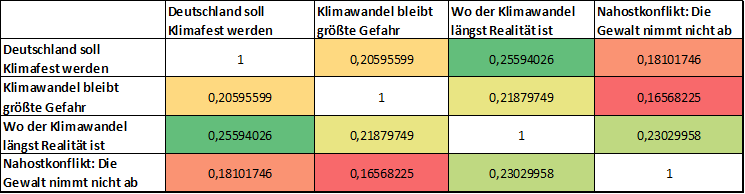
\includegraphics[clip,width=\linewidth]{images/tabelle_abstand_artikel_1.png}%
	}

	\subfloat[Mit Herausfiltern der Stoppwörter]{%
		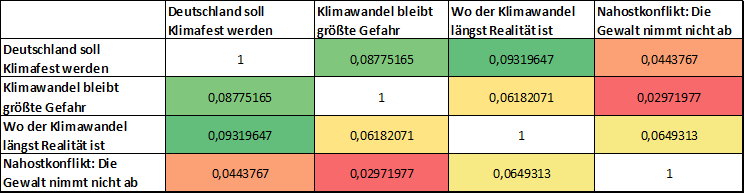
\includegraphics[clip,width=\linewidth]{images/tabelle_abstand_artikel_2.png}%
	}

	\subfloat[Mit Herausfiltern der Stoppwörter und Wortstammrückführung]{%
		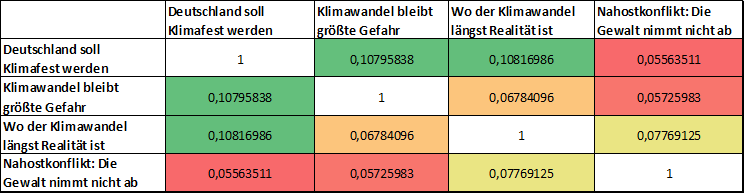
\includegraphics[clip,width=\linewidth]{images/tabelle_abstand_artikel_3.png}%
	}

	\subfloat[Mit Herausfiltern der Stoppwörter, Wortstammrückführung und Minimalanzahl für Wort]{%
		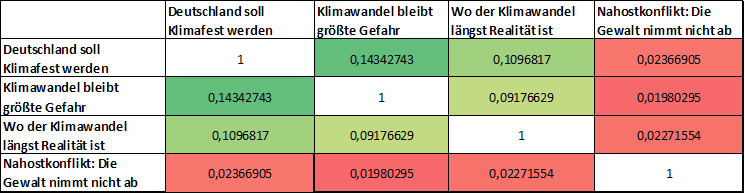
\includegraphics[clip,width=\linewidth]{images/tabelle_abstand_artikel_4.png}%
	}
	\caption{Ähnlichkeitsmaße der einzelnen Artikel unter Verwendung der Kosinus-Ähnlichkeit}
	\label{fig:textvergleich}
\end{figure}
\section{Vegleich von Kosinus-Ähnlichkeit zur euklidischen Distanz}
Die in Abbildung \ref{fig:textvergleich} gezeigten Werte wurden alle mit der Kosinus-Ähnlichkeit berechnet. Durch den nun beschriebenen Schritte wurde beschrieben, wie für einzelnen Texte Merkmalsvektoren so berechnet werden können, dass sie von anderen Texten unterscheidbar sind. Für die vier Texte wurden jeweils Merkmalsvektoren berechnet werden. Nun soll unter der Verwendung dieser eine Distanzmatrix erstellt werden, einmal mithilfe der Kosinus-Ähnlichkeit und einmal mithilfe der der euklidischen Distanz. Das in Abbildung \ref{fig:calcvergleich} abgebildete Ergebnis zeigt eindeutig, dass die Kosinus-Ähnlichkeit besser differenzierbare Werte liefert als die euklidische Distanz. Somit soll im weiteren die Kosinus-Ähnlichkeit verwendet werden.
\begin{figure}
	\centering
	
	\subfloat[Distanzmatrix berechnet mit der Kosinus-Ähnlichkeit]{%
		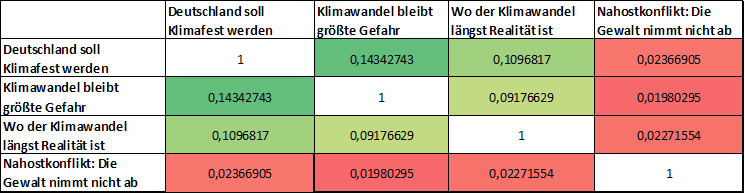
\includegraphics[clip,width=\linewidth]{images/tabelle_abstand_artikel_4.png}%
	}
	
	\subfloat[Distanzmatrix berechnet mit der euklidischen Distanz]{%
		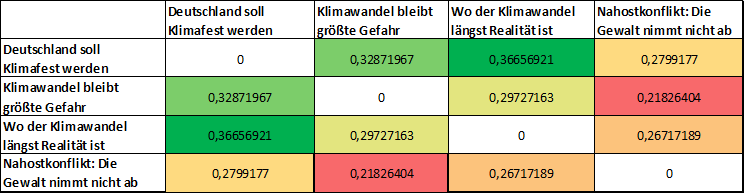
\includegraphics[clip,width=\linewidth]{images/tabelle_abstand_artikel_5.png}%
	}
	\caption{Differenzierbarkeit von Werten berechnet mithilfe der Kosinus-Ähnlichkeit im Vergleich zur euklidischen Distanz}
	\label{fig:calcvergleich}
\end{figure}
Nun muss der Prozess, der bei Tagesschauartikeln funktioniert auf die einzelnen Nutzer*innen angewendet werden. Ziel ist die Erstellung eines Merkmalsvektoren analog zu dem aus Formel \ref{eq:merkmalsvektoren}. 
\section{Erstellung der Merkmalsvektoren für Nutzer*innen}
Will man die Merkmalsvektoren der Nutzer*innen bestimmen, muss man zunächst die Schlüsselwörter aller Ihrer Texte zusammenführen, also alle Tweets, die von ihnen verfasst wurde. Die Schlüsselwörter werden anhand dem in den vorherigen Kapiteln beschriebenen Prozess aus dem Text extrahiert und um einen weiteren Filter ergänzt: Es werden nur Wörter in Betracht gezogen, welche als Hashtag markiert wurden. \\ \newline
Pro Nutzer*innen wird also für jeden der von ihm verfassten Tweets die Häufigkeitsverteilung der Schlüsselwörter berechnet und dann in eine große Häufigkeitsverteilung pro Nutzer*innen zusammengefasst. Die beinhaltet nun, welche Schlüsselwörter der Nutzer*innen wie Häufig über den gesamten Datensatz hinweg verwendet hat. In einem weiteren Schritt wird nun berechnet, wie oft ein Schlüsselwort im gesamten Datensatz vorkommt. Um den Datensatz zu reduzieren und so auch Rauchpunkte zu entfernen, sollen nun Schlüsselwörter, welche nicht sehr häufig verwendet werden, herausgefiltert werden. Da die Tweets nach einen bestimmten Thema ausgesucht wurden, werden Schlüsselwörter die dieses beinhalten unverhältnismäßig häufig auftauchen, dadurch wird auch ein Schwellwert für eine obere Grenze benötigt. Als geignet erwies sich, nur Wörter zu verwenden, deren Häufigkeit zwischen dem 97\% und dem 99.98\% Quantil der Häufigkeiten aller Wörter lagen. Somit werden 98\% aller möglichen Schlüsselwörter nicht betrachtet. Für einen Datensatz von einem Monat entspricht dies 404,905 Wörtern. \\ \newline
Weiterhin sollen für den einzelnen Nutzer*innen auch nur die Wörter verwendet werden, welche er häufig verwendet. Hierfür wird zunächst eine Liste gebildet, welche  für jeden Nutzer*innen und jedes Wort beinhaltet, wie häufig der Nutzer*innen dieses Wort verwendet hat. Als Schwellwert dient das 99\% Quantil dieser Liste verwendet, welches bei den Tweets eines Monats bei sechs liegt. Nutzer*innen, welche mit keinem ihrer Schlüsselwörter diesen Schwellwert erreichen, werden ausgefiltert. Durch beide Filterschritte zusammen fallen 99.5\% der Nutzer*innen aus dem Datensatz, was für einem Monat eine Zahl von 238.717 Nutzer*innen entspricht. Der gesamte Prozess ist in Abbildung \ref{fig:merkmalsvektoren} zusammengefasst.\\ \newline
\begin{figure}[h]
	\centering
	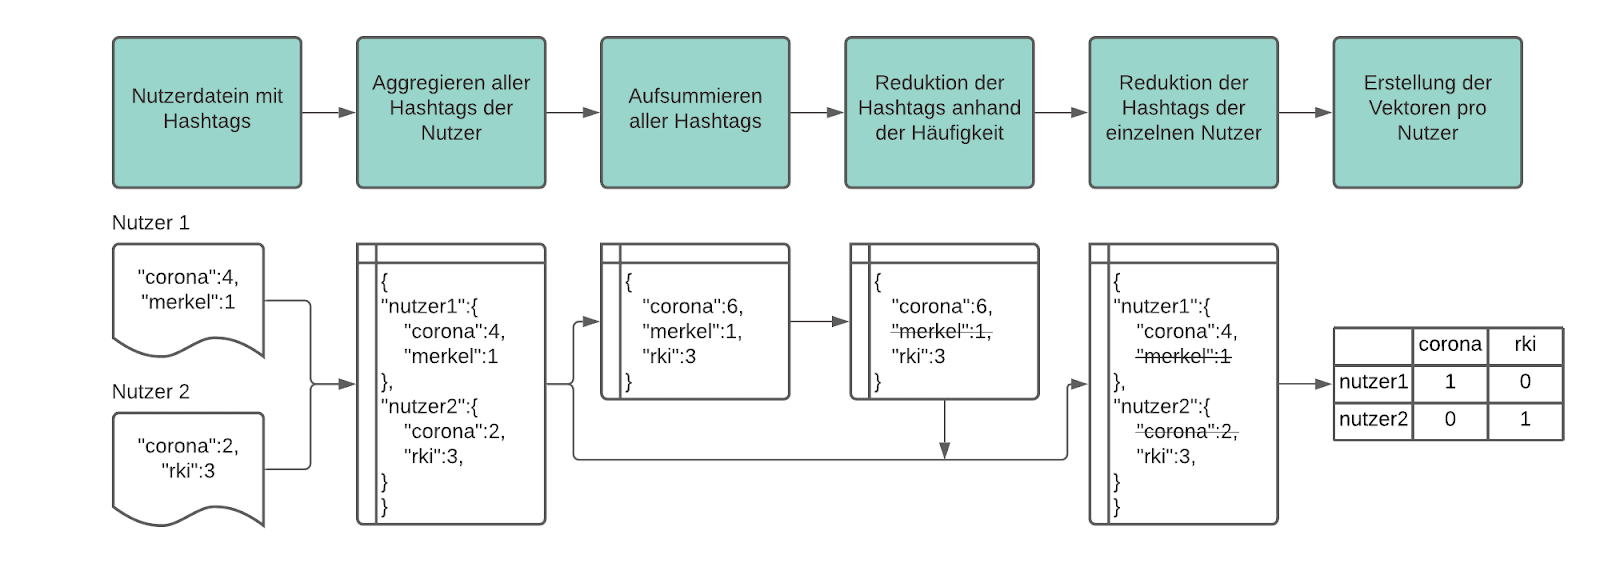
\includegraphics[width=\linewidth]{images/vergehen_merkmalsvektoren_nutzer}
	\caption[]{Bestimmung der Merkmalsvektoren der Nutzer*innen}
	\label{fig:merkmalsvektoren}
\end{figure}
\subsection{Clustering anhand der Merkmalsvektoren}
Da nun für jede*n Nutzer*in ein Merkmausvektor bekannt ist, soll nun versucht werden, die Nutzer*innen anhand dieser in Kategorien einzuteilen. Der Prozess soll analog zum Clustering aus \cite{Godfrey.21.08.2014} erfolgen: Es soll zunächst durch mehrere Iterationen des $k$-Means Algorithmus eine Ähnlichkeitsmatrix gebildet werden, anschließend soll das Ergebnis mithilfe dieser und dem DB-SCAN Algorithmus zusammengefasst werden. 
\subsubsection{Berechnung einer Ähnlichkeitsmatrix mithilfe des k-Means Algorithmus}
Der k-Means Algorithmus ist ein sehr bekannter Algorithmus, mit dem Ziel, n Merkmalsträger in k Cluster zu partitionieren, in denen jede Beobachtung zu dem Merkmalsträger mit dem nächstgelegenen Mittelwert (Clusterzentren oder Clusterschwerpunkt) gehört, der als Prototyp des Clusters dient. Allerdings birgt er auch Probleme: Dadurch, dass die Clusterzentren am Anfang zufällig gewählt werden kann der Algorithmus bei gleiche Eingabe einen ungleiches Ergebnis. Abbildung \ref{fig:kmeans} visualisiert dieses Verhalten. Zudem muss bei diesem Algorithmus die Anzahl an zu findenden Clustern vorgegeben werden. Dies kann insofern zu nicht optimalen Ergebnissen führen, da sich der Datensatz potentiell sinnvoller in eine Anzahl von Clustern unterteilen lässt, welche ungleich k ist. 
\begin{figure}[h]
	\centering
	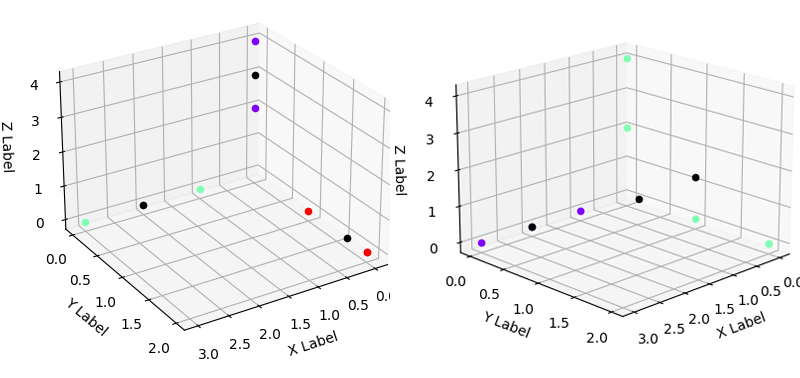
\includegraphics[width=\linewidth]{images/gutes_schlechtes_kmeans}
	\caption[]{Gutes (links) und schlechtes (rechts) Ergebnis des k-Means Algorithmus unter gleichem Input}
	\label{fig:kmeans}
\end{figure}
Für jeden Lauf von k-means wird der Wert innerhalb der Matrix bei (Benutzer A, Benutzer B) und (Benutzer B, Benutzer A) um einen dieser Benutzer erhöht, der im selben Cluster in demselben Cluster landen. Daraus ergibt sich eine Matrix, anhand derer man für jeden Benutzer sagen kann, wie oft er mit einem anderen Benutzer geclustert wurde einem anderen Benutzer geclustert wurde und somit, wie ähnlich die Eigenschaften der die Benutzer sind.
\subsubsection{Einteilung der Nutzer mit dem DB-SCAN Algorithmus}
Durch die Verwendung der Ähnlichkeitsmatrix und die Anwendung des DB-SCAN
Algorithmus können nun die Benutzer*innen nun in verschiedene Cluster eingeteilt werden.
Darüber hinaus bietet dieser Algorithmus die Möglichkeit
Benutzer, die sich nicht in einem ausreichenden Agglomerationszentrum befinden
Zentrum liegen, als Rauschpunkte zu markieren, anstatt sie einem Cluster zuzuordnen.
In diesem Fall hängt epsilon von der Anzahl der Iterationen mit
k-means ab, da diese definiert, wie oft ein Benutzer maximal
durch den k-means-Algorithmus geclustert werden kann. Epsilon wird gesetzt auf
80 % dieses Wertes. Die Anzahl der minimalen Benutzer zur Bildung eines
Cluster zu bilden, ist definiert durch die Anzahl der Benutzer im Datensatz
mal 0,02.

